% additions.tex -- text for main.tex, 2026-10-02.  Each block says where it goes.
% Blocks A-C are ready.  Block D (off-diagonal sector) is a skeleton awaiting the c_j = 0 run.
% Numbers: NOTE_2d.md, NOTE_rung1.md, hdym_analytic.py (sympy, every constant checked).

% =====================================================================================
% A.  Sec. 5.2 "Channel statistics".  REPLACES the sentences from "This can be checked
%     quantitatively at the level of the tail constant." to "...is the whole story."
% =====================================================================================

This can be checked quantitatively at the level of the tail constant, and the detuned share can
be derived. Equation (\ref{eq:tail}) gives $A_{\rm res}=32\pi I\nu_0=6.14$ for the resonant
$x$-channel share of $\hat s_{xx}$. The remainder comes from the $y$- and $z$-channels, in two
ways. During a $y$-channel visit the entry $z^2$ chirps directly, with amplitude $J_z/D$ at
frequency $2|y|$. In addition the along-channel coordinate is not slow at second order: the
transverse oscillators exert the force $-\partial_yV=-y(x^2+z^2)=-\mathrm{sgn}(y)\sum_a
J_a(1+\cos2\phi_a)$ on $y$, whose oscillating part produces the response
$\delta y=\mathrm{sgn}(y)\sum_aJ_a\cos2\phi_a/(4y^2)$ and hence a term
$2y\,\delta y=(J_x\cos2\phi_x+J_z\cos2\phi_z)/(2D)$ in $K_{xx}=y^2+z^2$, at the same frequency
$2|y|$. The $\phi_z$ pieces are coherent, so the oscillating part of $K_{xx}$ in the $y$-channel
is $(3J_z/2D)\cos2\phi_z+(J_x/2D)\cos2\phi_x$, with power $(9J_z^2+J_x^2)/4D^2$ once the
independent phases are averaged; the $z$-channel contributes $(9J_y^2+J_x^2)/4D^2$. The uniform
measure on the two transverse actions makes all $\langle J_a^2\rangle$ equal and the three
channels equally visited, so resonant\,:\,detuned\,:\,total $=2:5:7$,
\begin{equation}
A=\tfrac72A_{\rm res}=21.5,\qquad \frac{A_{\rm res}}{A}=\frac27=0.286,
\label{eq:seven}
\end{equation}
against the measured $A=21.6\pm0.3$ of (\ref{eq:A}). The detuned $5/7$ of the tail power sits at
frequency $2|y|$ or $2|z|$ while $w_x$ has frequency $\sqrt{1+y^2}\approx|y|$ or $\sqrt{1+z^2}$
during those visits, detuned from its parametric resonance by $\sim1/D$ against a half-width
$\lesssim1/(2D^3)$; it drives nothing. If only the resonant share drives the ghost, the ratio of
the measured diagonal-ghost exponent to the prediction of (\ref{eq:spectral}) applied to the
\emph{full} measured spectrum should be $2/7$. It is $0.283$, $0.285$, $0.290$, $0.276$ at
$E=0.008$, $0.015$, $0.02$, $0.03$ (Table~\ref{tab:low}; and $0.15$ at $E=0.05$, where $u=4.2$ is
below the onset of the $u^{-6}$ regime). The tail is entirely channel power, its composition is
derived, and (\ref{eq:law}), which counts only the resonant piece, is the whole story. The same
accounting gives the tail constant of any entry of $\Hess V$; for the decoupled component studied
in Sec.~\ref{sec:twofield} below it predicts $\tfrac92A_{\rm res}$, measured $4.3$--$4.4$.

% -------------------------------------------------------------------------------------
% A'. Sec. 2 "The model", after "...the energies quoted below are energy densities, the total
%     energy on the torus being $L^3E$."  ADD:
% -------------------------------------------------------------------------------------
Throughout, $E$ is the energy of the Yang--Mills background. On the ghost-free manifold it is
the total energy of the system, and the linearised ghost of (\ref{eq:hill}) does not change it;
the full Lee--Wick energy is indefinite, and in the nonlinear runs of Sec.~\ref{sec:nonlinear}
$E$ refers to the Yang--Mills energy of the initial data, the ghost being seeded at amplitude
$\delta$.

% =====================================================================================
% B.  NEW SUBSECTION at the end of Sec. 5 (after Eq. (\ref{eq:final}) and its discussion).
% =====================================================================================

\subsection{The exponent as a count of transverse actions; test on the two-field model}
\label{sec:twofield}

Nothing in the derivation is specific to three degrees of freedom. For a diagonal potential
$V=\tfrac12\sum_{i<j}q_i^2q_j^2$ with $N=n+1$ degrees of freedom, so that a channel has $n$
transverse actions, the microcanonical entry flux is $\nu_0=2(2\pi)^n/Z_N$ per channel, the
passage integral is the Dirichlet integral
$I_n=\int_{\sum a<1}(\sum a_i^2)\,[2(1-\sum a)]^{-1/2}d^na=\sqrt{2\pi}\,n/\Gamma(n+\tfrac52)$,
and
\begin{equation}
\lambda_{\rm diag}=\frac{\pi}{16}I_n\nu_0\,E^{(n+7)/4}
=\frac{2^{\,n-5/2}\pi^{n+3/2}\,n}{\Gamma(n+\frac52)}\;\frac{E^{(n+7)/4}}{Z_N},
\qquad \frac{A_{\rm res}}{A}=\frac{4}{9n-4},
\label{eq:general}
\end{equation}
which reduces to (\ref{eq:final}) and (\ref{eq:seven}) at $n=2$. The exponent decomposes as
$\tfrac34$ (kinematic) $+\,\tfrac n4$ (the measure of $n$ small actions is $\propto J^n$)
$+\,1$ (driving power $\propto(J/D)^2$); the middle term is the only one that knows $N$. The
$n=1$ case is the two-field $x^2y^2$ model, which is the invariant plane $z=0$ of the present
system, i.e.\ the ansatz $A^a_i={\rm diag}(x,y,0)$, with prediction $\lambda\propto E^2$ and
prefactor $2\sqrt2\pi^2/15=1.861$ over $Z_2$, and a predicted resonant share of $4/5$.

The two-field model needs one modification: in two dimensions the channel cross-section falls as
$1/|x|$ rather than $1/x^2$, so the classical density of states is logarithmically divergent
\cite{Simon83}, the mean channel-visit time $\int dJ/J$ diverges, and every time average,
including $\lambda_\YM$, decays as $1/\ln T$. We close the channels with a mass,
$V=\tfrac12x^2y^2+\tfrac12\mu^2(x^2+y^2)$ with $\mu^2=\mu_1^2E^{1/2}$, which keeps the model
exactly scale-free (every energy is the rescaled $E=1$ system with regulator $\mu_1$) and makes
$Z_2(\mu_1)=8\sqrt2\pi\sqrt{1+b^2}\,[K(m)-E(m)]$, $b^2=\mu_1^4/2$, $m=1/(1+b^2)$, finite:
$Z_2=189.7$ at $\mu_1=0.1$ and $275.3$ at $\mu_1=0.03$. The regulator enters the passage
integral through the turning-point condition $JD+\tfrac12\mu^2D^2=1$, which multiplies the
prediction by $(1-\mu_1^2/2\sqrt E)^{5/2}$ ($0.88$ at $E=0.01$, $\mu_1=0.1$), and shifts the
ghost mass to $1+\mu^2$, a $1\%$ effect. Every ingredient was checked separately at $E=1$: the
flux $\nu_0=4\pi/Z_2$ is reproduced to $0.3\%$ at both $\mu_1$ by $6\times10^4$ channel visits,
the entry measure is uniform in $J$, $DJ+\tfrac12\mu^2D^2=1.000$ at the turning point, and the
measured tail $u^5\hat s_{xx}$ is $(1.25\pm0.02)\times A_{\rm res}(1-\mu^2D^2/2)^{5/2}$, flat
over $u=8$--$45$, the $5/4$ being the $n=1$ value of (\ref{eq:general}).

\begin{table}
\centering
\caption{Two-field model: diagonal-ghost exponent against the parameter-free prediction
(\ref{eq:general}) with $n=1$ and the regulator factors ($N=10^5$ at $E=0.1$, $2\times10^5$
otherwise). $\lambda_z$ is the exponent of the decoupled third component $w_z$, driven by
$K_{zz}=x^2+y^2$, all of whose channel power is detuned.}
\label{tab:twofield}
\begin{tabular}{cccccc}
\toprule
$E$ & $\mu_1$ & $\lambda_{\rm diag}$ & prediction & ratio & $\lambda_z/\lambda_{\rm diag}$\\
\midrule
$0.1$  & $0.1$  & $8.08\times10^{-5}$ & $9.32\times10^{-5}$ & $0.87$ & $0.235$\\
$0.03$ & $0.1$  & $7.76\times10^{-6}$ & $8.15\times10^{-6}$ & $0.95$ & $0.017$\\
$0.01$ & $0.1$  & $8.85\times10^{-7}$ & $8.60\times10^{-7}$ & $1.03$ & $0.005$\\
$0.03$ & $0.03$ & $5.75\times10^{-6}$ & $6.04\times10^{-6}$ & $0.95$ & $0.015$\\
\bottomrule
\end{tabular}
\end{table}

Table~\ref{tab:twofield} gives the result. The local slope between $E=0.03$ and $0.01$ is
$1.98$ against the predicted $2.05$ (including the energy dependence of the regulator factor),
and the prefactor is reproduced to $5\%$ at $u=4.8$ and $3\%$ at $u=6.3$, approaching the
asymptote from below exactly as the three-field data do at the same $u$. Changing $\mu_1$ from
$0.1$ to $0.03$ changes $Z_2$ by $45\%$ and the regulator correction by $7\%$; the ratio to
prediction is $0.951$ in both cases, which tests the $1/Z$ factor in a way the three-field model
cannot. With the measured spectrum in (\ref{eq:spectral}) the ghost sees $0.83$ of the tail
power at $E=0.03$ and $0.01$, against the predicted $4/5$. Finally $\lambda_z/\lambda_{\rm diag}$
falls from $0.235$ to $0.005$ between $E=0.1$ and $0.01$, faster than any power: detuned
channel power is inert, as assumed throughout. The decomposition of the exponent is therefore
tested at $n=1$ and $n=2$, and the single number left in (\ref{eq:general}) that is not a closed
form is the density of states $Z_3=557.1$. Within the adiabatic and weak-driving approximations
the law is exact given ergodicity of the Yang--Mills flow on the energy shell, with corrections
$O(E^{1/2})$; the $5\%$ at $u=4.8$ in both models is what that looks like.

% =====================================================================================
% C.  Discussion, "Open items": REPLACE item (ii) and renumber.
% =====================================================================================

\paragraph{Open items.} (i) The vector/diagonal factor ($\simeq2.2$ at $E=0.015$--$0.03$,
$1.75$ at $E=0.008$): a derivation of the mode-mixing contribution and of the rate at which it
dies off, which would turn the asymptotic statement into a prediction for the physical ghost at
all $E\lesssim0.03$. (ii) The finite-time Lyapunov distribution of the full flow,
whose tail sets $\alpha$ (Sec.~\ref{sec:nonlinear}). (iii) The regular islands as a possible
positive-measure refuge. (iv) The rate law of the off-diagonal ghost sector
(Sec.~\ref{sec:offdiag}), whose derivation is the natural sequel to this paper. (v) Bianchi IX
minisuperspace of quadratic gravity, in which the same calculation can be done for the theory of
actual interest.

% Also: in the abstract, "The two-field ... (ii)" no longer applies; and Sec. 2 "The model" could
% cite Sec. \ref{sec:twofield} after "(the same integral underlies the discreteness...)".

% =====================================================================================
% D.  SKELETON -- new Section after "Invariant sets" and before "Discussion".
%     Numbers are final; the mechanism paragraph waits for the c_j = 0 run.
% =====================================================================================

\section{The off-diagonal ghost sector}
\label{sec:offdiag}

The colour-diagonal ansatz is a consistent truncation, but the Lee--Wick ghost of the full
homogeneous theory has nine components, of which the ansatz keeps three. Linearising the full
homogeneous system (all nine $A^a_i$, $A_0=0$) about a diagonal ghost-free solution, the six
off-diagonal components $u^a_i$ ($a\ne i$) split exactly into three equivalent blocks
$(u_{12},u_{21})$, $(u_{13},u_{31})$, $(u_{23},u_{32})$, with quadratic Lagrangian
\begin{equation}
L_2=\tfrac12|\dot u|^2-\tfrac12u^{\rm T}m\,u-\tfrac12|\ddot u+m\,u|^2+\tfrac12j^2,\qquad
m=\begin{pmatrix}z^2&-xy\\-xy&z^2\end{pmatrix},\quad
j=x\dot u_{12}-y\dot u_{21}-\dot x\,u_{12}+\dot y\,u_{21},
\label{eq:L2}
\end{equation}
for the first block. The first three terms are the structure of (\ref{eq:Lred}) with $m$ the
corresponding block of the Hessian of the nine-dimensional Yang--Mills potential; the last is
the $(D^\mu F_{\mu0})^2$ piece of the Lee--Wick action, $j$ being the linearised colour charge
$(A_i\times\dot A_i)_3$. It vanishes identically on the ansatz and is why (\ref{eq:Lred}) has no
such term. Each block carries one exact gauge zero mode $u=\theta\times A$, one conserved
linearised Gauss charge, and three physical degrees of freedom: one of Yang--Mills type and two
ghosts, the second ghost being the longitudinal polarisation of the massive vector, which has no
diagonal counterpart (in a channel the two sit at frequencies $1$ and $\sqrt{1+x^2}$, the $j^2$
term lifting the second). The count is $6+9$ for the full homogeneous theory, as it must be.

Two facts follow. First, the off-diagonal Yang--Mills directions are neutral. The singular-value
decomposition $A^a_i=(O_{\rm c}\,{\rm diag}(x,y,z)\,O_{\rm s})^a_i$ identifies them as the three
colour rotations, which are gauge, and the three spatial rotations, whose generators $J_{ij}$ are
conserved; the diagonal ansatz is the $J=0$ sector of homogeneous Yang--Mills mechanics, not a
measure-zero slice of a larger chaotic system. The linearised Yang--Mills block has two conserved
linear functionals and a zero mode, forcing all four of its exponents to vanish; numerically they
are $\pm\ln T/T$. The homogeneous theory therefore has no ``generic'' background beyond the one
studied here, and the fragmentation referred to in Sec.~\ref{sec:discussion} is an inhomogeneous
effect only.

Second, the off-diagonal ghost grows faster than the diagonal one, and with a different law.
Table~\ref{tab:offdiag} gives the two positive Lyapunov exponents of the block along
Yang--Mills backgrounds at five energies ($N=2\times10^4$--$2\times10^5$ trajectories, two
vectors with Gram--Schmidt, same estimator as Sec.~\ref{sec:methods}).

\begin{table}
\centering
\caption{Off-diagonal ghost exponents $g_1\ge g_2$ of one block of (\ref{eq:L2}), statistical
errors $\le0.3\%$, against the diagonal single-mode law (\ref{eq:final}).}
\label{tab:offdiag}
\begin{tabular}{cccccc}
\toprule
$E$ & $g_1$ & $g_2$ & $g_1/g_2$ & $g_1/(0.0120E^{9/4})$ & local slope of $g_1$\\
\midrule
$1$    & $1.180\times10^{-2}$ & $5.88\times10^{-3}$ & $2.01$ & $0.98$ & \\
$0.3$  & $3.371\times10^{-3}$ & $1.73\times10^{-3}$ & $1.95$ & $4.2$ & $1.04$\\
$0.1$  & $6.155\times10^{-4}$ & $3.94\times10^{-4}$ & $1.56$ & $9.1$ & $1.55$\\
$0.03$ & $2.625\times10^{-4}$ & $1.46\times10^{-4}$ & $1.80$ & $58$ & $0.71$\\
$0.01$ & $1.326\times10^{-4}$ & $7.75\times10^{-5}$ & $1.71$ & $349$ & $0.62$\\
\bottomrule
\end{tabular}
\end{table}

The exponent is not a single power law: the local slope falls from $1.5$ to $0.6$ between
$E=0.3$ and $0.01$, far below the $9/4$ of the diagonal sector and below the $5/4$ that the
$u^{-2}$ tail of the off-diagonal Hessian entry $xy$ would give if it drove a degenerate ghost
pair resonantly. At $E=0.01$ the off-diagonal ghost grows $350$ times faster than the diagonal
one, and the ratio increases roughly as $E^{-1.6}$.
%
The mechanism can be isolated by switching off the $(D^\mu F_{\mu0})^2$ term ($c_j=0$ in the
code). Then $m=z^2\mathbf 1-xy\,\sigma_x$ has the fixed eigenvectors $(1,\pm1)$ and the pair
decouples exactly into two scalar Hill equations $\ddot w_\pm=-(1+z^2\mp xy)\,w_\pm$. In the
$x$-channel the entry $xy=\sqrt{2J_y|x|}\cos\phi_y$ chirps at frequency $|x|$, not $2|x|$, with an
amplitude that is not suppressed by depth, so it meets the parametric resonance at $|x|=2$; and
because without the $j^2$ term both $w_\pm$ keep frequency $\simeq1$ in every channel, the
$y$-channel resonates as well. The passage integral of Sec.~\ref{sec:channels} with one power of
$J$ gives $u^2\hat s_{xy}=16\sqrt2\pi\nu_0/15=0.672$ (measured $0.68$--$0.72$ over $u=4$--$20$
along $E=1$ trajectories) and
\begin{equation}
\lambda_\pm=\frac{4\sqrt2\,\pi^3}{15}\,\frac{E^{5/4}}{Z}=0.0210\,E^{5/4},
\label{eq:fivequarters}
\end{equation}
the $u^{-2}$ tail noted in Sec.~\ref{sec:channels} turned into a rate. Measured with $c_j=0$:
$g_1=g_2$ to $5\%$, $5.07\times10^{-3}$ at $E=0.3$ and $1.47\times10^{-3}$ at $E=0.1$ against
$4.66\times10^{-3}$ and $1.18\times10^{-3}$, with $75\%$ of the growth at $E=0.1$ in the $27\%$
of the time spent in channels; the excess is the knee of the $xy$ spectrum at $u\le3.6$ and a
modulation depth $\sqrt{2E}$ that is not yet small. In the actual theory the $j^2$ term lifts the longitudinal ghost to frequency $\sqrt{1+x^2}$
inside a channel and detunes this resonance, which is why $g_1$ is $2.5$ times smaller than
(\ref{eq:fivequarters}) at $E=0.1$ and $g_1\ne g_2$. The growth nevertheless stays in the
channels: at $E=0.1$, $79\%$ of the log-growth of the leading vector accrues in the $27\%$ of the
time spent at depth $D>3$, the same split as with $c_j=0$. What changes with the energy is the
character of the events. Figure~\ref{fig:Q} shows $Q=\sigma^2T/\lambda$, the variance of the
per-trajectory finite-time exponent times the run length over its mean, which for growth that
arrives in discrete passages is the typical log-gain per passage and is independent of $T$.
Every parametric mechanism in this paper gives $Q\simeq1$--$3$, flat in $E$: the diagonal ghost,
the two-field model, and the $c_j=0$ block. The off-diagonal ghost of the actual theory climbs as
$Q\simeq1.9E^{-1/2}$ from $E=0.3$ down, reaching $19$ at $E=0.01$ while fewer than $0.2\%$ of
trajectories have a negative finite-time exponent: its growth comes in rare deep channel visits
during each of which the ghost gains $e^{19}$. That is not the small kick per passage of
parametric resonance but an instability that persists for the duration of a visit, and the
shallow energy dependence of Table~\ref{tab:offdiag} is its measure of deep visits. The only
term of (\ref{eq:L2}) whose frozen coefficients can change sign inside a channel is the
Gauss-charge term, which is where a derivation would start; we leave it to a sequel
(Sec.~\ref{sec:discussion}).

\begin{figure}
\centering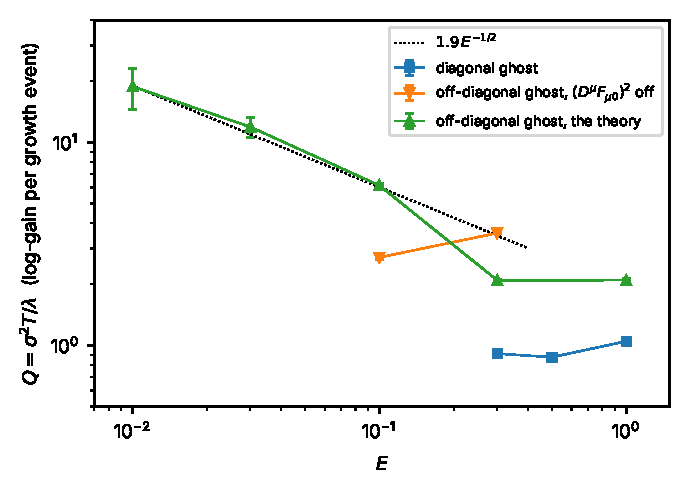
\includegraphics[width=.6\textwidth]{fig_Q.pdf}
\caption{Log-gain per growth event, $Q=\sigma^2T/\lambda$, from the per-trajectory finite-time
exponents of every production run. The parametric mechanisms (diagonal ghost, two-field model,
off-diagonal block with the Gauss-charge term off) give $Q$ of order one, independent of $E$;
the off-diagonal ghost of the actual theory climbs as $E^{-1/2}$ (dotted). The diagonal point at
$E=0.008$ is the run whose extrapolation uncertainty is $10\%$ (Table~\ref{tab:low}).}
\label{fig:Q}
\end{figure}

The consequence for the headline result is a strengthening with a change of scope:
(\ref{eq:final}) is the law of the colour-diagonal ghost, and the transverse exponent of the
ghost-free manifold of the full homogeneous theory is set by the off-diagonal sector, which is
less benign at every energy below $E\simeq1$ and increasingly so as $E\to0$. There is still no
threshold and no exponential suppression.

% Scope paragraph of the Discussion: replace "On a large torus the homogeneous Yang--Mills
% condensate is itself unstable to inhomogeneous modes at rates of order $\lambda_\YM$" with
% "Within the homogeneous sector the diagonal ansatz is neutral (Sec.~\ref{sec:offdiag}); on a
% large torus the homogeneous condensate is unstable to inhomogeneous modes at rates of order
% $\lambda_\YM$" -- the rest stands.
% Abstract: after "...no exponential suppression." add one sentence: "The six ghost components
% that the diagonal ansatz discards grow faster still, by a factor that reaches 350 at
% $E=0.01$, with a shallower energy dependence; with the $(D^\mu F_{\mu0})^2$ term switched off their
% law is derived, $0.0210\,E^{5/4}$."
